\begin{frame}{Why Stochastic Policies? The Aliased Grid World}
\begin{figure}
\centering
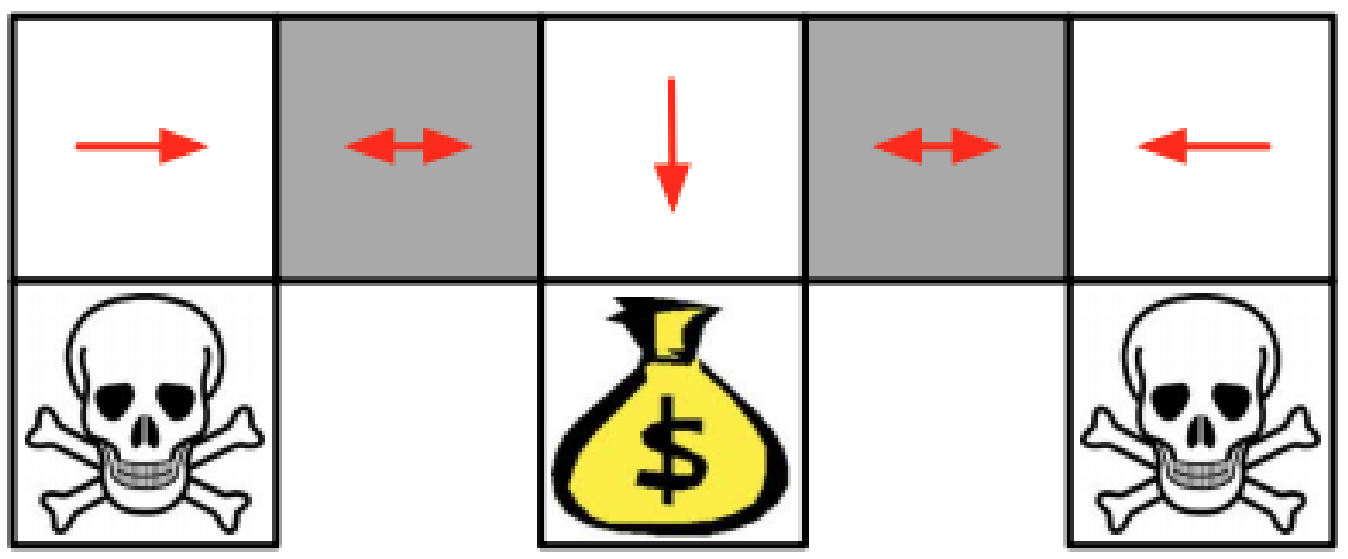
\includegraphics[width=0.6\textwidth,height=0.33\textheight,keepaspectratio]{images/vanilla-policy-gradient/grid_world_3.png}
\end{figure}
\begin{itemize}
    \item Grey states are \textbf{aliased}: the agent observes the same features in multiple distinct positions
    \item A deterministic policy must make the same choice in every grey state --- always go East or always go West --- causing the agent to get stuck in a loop and never reach the goal
    \item A \textbf{stochastic} 50/50 policy breaks the symmetry: the agent eventually reaches the goal with probability 1
    \item This is the concrete motivation for the softmax and Gaussian parameterisations on the previous slide
\end{itemize}
\end{frame}
